\begin{multicols}{3}[\section{3G}]

\rhead{Henrik Scholl, Johannes Hill}
\lfoot{18.05.2016}

\newrefsegment

\begin{tabular}{p{2,1 cm}p{2.7 cm}}
\textbf{Steckbrief}& \\
\end{tabular}
\rowcolors{1}{\topicolor!20}{}
\begin{tabular}{p{2,1 cm}p{2.7 cm}}
      Einsatz seit & Oktober 2000\\
      Frequenz"-bereich  & \SI{5}{\mega\hertz}\\
      Datenrate & \SI{14,4}{Mbit/s}\\
      Verbreitung & Weltweit\\
      Reichweite & Global\\
      Modulation & Frequency Division Multiplex, \newline Time Division Multiplex\\
\end{tabular}
\par
%Source http://www.fh-bingen.de/fileadmin/user_upload/Lehrende/Kilsch_Dieter/internet/projekte/TedoSchStiUnits.pdf -> Seite 9 findet ihr alle verwendbaren Einheiten, wie:
%\SI{Zahl}{\mega\hertz} oder \SI{Zahl}{\mili\metre}
%Ich weiß ehrlich gesagt nicht welche Einheiten ihr im Text genau braucht, aber in dem Dokument und mit obigen Beispiel sollte es umsetzbar ein.
\subsection*{Überblick}
\begin{wrapfigure}{r}{0.4\linewidth}
  \vspace{-20pt}
  \begin{center}
  	\hspace{-20pt}
    
\includegraphics[width=0.7\linewidth]{Kapitel/3G/Grafiken/umts_logo.png}
  \end{center}
  \vspace{-15pt}
\end{wrapfigure}
3G oder auch \textbf{UMTS} (\textbf{U}niversal \textbf{M}obile \textbf{T}elecommunications \textbf{S}ystem) wird als dritte Generation des Mobilfunkstandards bezeichnet und ist somit die Weiterentwicklung des GPRS-Dienstes. Bereits im Jahr 2000 konnte Deutschland die Lizenzen an dieser Technologie für den damaligen Preis von 98,8 Milliarden DM erwerben. Innerhalb Deutschland wurden diese Lizenzen an sechs Mobilfunkbetreiber für einen Preis von je 16 Milliarden DM weiterverkauft. Weitere Informationen zu diesem Sachverhalt finden sie in dem Abschnitt Anbieter und Gremien. 

Der große Durchbruch war der Technologie bei der Einführung in den Markt nicht vergönnt. Aufgrund hoher Kosten für den Endnutzer wurde nur zögerlich zur 3G-Technologie gegriffen. Auch für die Firmen war der Einstieg in dieses Segment nicht einfach. Durch die hohen Lizenzkosten schwand die Liquidität der Firmen und dies hatte einen Wertverlust an der Börse zur Folge. Auch die ausbleibenden Nutzer waren anfangs ein Problem. Zusammenfassend lässt sich sagen, dass die hohen Lizenzgebühren einen zügigen Netzausbau verhinderten. Erst 2003 konnten die ersten Probeläufe mit einigen Firmenkunden unternommen werden und ab 2004 wurde es in Deutschland kommerziell genutzt. 
 
Die Weiterentwicklung von UMTS wurde mit der Implementierung des Protokolls \textbf{HSPA} (\textbf{H}igh \textbf{S}peed \textbf{P}acket \textbf{A}ccess) realisiert. Da HSPA einen Fortschritt gegenüber UMTS darstellt, aber auf derselben Basis arbeitet, wird es nicht als 4G Netz sondern als 3.5G oder auch 3G+ bezeichnet. Den deutschen Markt erreichte HSPA erst Anfang 2006 und wurde noch im gleichen Jahr für einige Geschäftskunden zur Verfügung gestellt. ~\cite{3G.1, 3G.2}

\subsection*{Technische Erläuterung}
\subsubsection*{UMTS}
Technisch gesehen ist UMTS eine Weiterentwicklung der GSM/GPRS-Architektur, welche anfänglich nur durch eine veränderte Software, bei gleichbleibenden Kernnetz, entstand. Das Zugangsnetz hingegen ist eine Neuentwicklung mit dem Namen \textbf{U}MTS \textbf{T}errestrial \textbf{R}adio \textbf{A}ccess \textbf{N}etwork (\textbf{UTRAN}). Die UMTS-Referenzarchitektur besteht aus insgesamt drei Bereichen oder auch Domains (siehe Abb. \ref{fig:domains}):
\begin{itemize}
	\item \textbf{U}ser \textbf{E}quipment \textbf{D}omain (\textbf{UED})
	\item \textbf{U}niversal \textbf{S}ubscriber \textbf{I}dentity \textbf{M}odule \textbf{D}omain (\textbf{USIMD}) 
	\item \textbf{M}obile \textbf{E}quipment \textbf{D}omian (\textbf{MED})
\end{itemize}
Die UED ist in die zwei Bereiche USIMD und MED untergliedert. Diese Domains beschreiben die Endgeräte, welche eine SIM-Karte besitzen. Die UED ist für die Authentisierung zuständig und über eine Luftschnittstelle Uu mit der \textbf{A}ccess \textbf{N}etwork \textbf{D}omain (\textbf{AND}) verbunden. 
 
Die AND wird bei UMTS durch UTRAN umgesetzt und ermöglicht die Ankopplung eines Mobiltelefons an das Core Network. Der Aufbau von UTRAN besteht aus mehreren \textbf{R}adio \textbf{N}etwork \textbf{S}ubsystems (\textbf{RNS}). Diese werden jeweils von einem \textbf{R}adio \textbf{N}etwork \textbf{C}ontroller (\textbf{RNC}) gesteuert. Hierbei hat der RNC mehrere Aufgaben, wie beispielsweise die Ver – und Entschlüsselung, die Staukontrolle sowie weitere Verwaltungsaufgaben. Ein solcher RNC verwaltetet hierbei einen oder mehrere Node B (Basisstationen), wobei eine solche Node B eine oder mehrere Antennen steuert. Die Antennenanzahl bedingt dann wiederum das Aufspannen einer oder mehrerer Funkzellen.

Die \textbf{C}ore \textbf{N}etwork \textbf{D}omain (\textbf{CND}) ist auch als Kernnetz bekannt und ermöglicht Verbindungen in das eigene Netz oder in andere Systeme. Hierbei wird die CND nochmals in \textbf{S}erving \textbf{N}etwork \textbf{D}omain (\textbf{SND}), \textbf{H}ome \textbf{N}etwork \textbf{D}omain (\textbf{HND}) und \textbf{T}ransit \textbf{N}etwork \textbf{D}omain (\textbf{TND}) aufgeteilt. In diesen Bereichen wird das Routing, die Lokalisierung, das Roaming, das Billing und das Charging umgesetzt. Weiterhin wird das Kernnetz in zwei weitere Bereiche eingeteilt. Einmal in die Circuit Swiched Domain, welche zur Leitungsvermittlung dient und andererseits in die Packet Switched Domain, die zur Paketvermittlung dient. Diese Unterscheidung beruht auf der Wahl der Dienste, die genutzt werden. So sind Datendienste, wie z.B. das Verschicken eines Bildes, auf die Paketvermittlung und Telefongespräche auf eine Leitungsvermittlung angewiesen. Eine solche Trennungen der beiden Domains ist oftmals nur Modellhaft. Die tatsächliche Umsetzung besteht lediglich nur aus einem Bauteil. Eine weitere Aufgabe des Kernnetzes ist die Verwaltung von mehreren \textbf{M}obile-Service \textbf{S}witching \textbf{C}entre (\textbf{MSC}) beziehungsweise \textbf{S}erving \textbf{G}PRS \textbf{S}upport \textbf{N}odes (\textbf{SGSN}) in den einzelnen RNS. Hierbei verwaltet nun jede MSC zusätzlich eine \textbf{H}ome \textbf{L}ocation \textbf{R}egister (\textbf{HLR}), welches die Nutzerdaten und ein \textbf{V}isitor \textbf{L}ocation \textbf{R}egister (\textbf{VLR})  beheimatet (siehe Abb. \ref{fig:architektur}).

Die Direct-Sequence-CDMA-Technik stellt einen wesentlichen Unterschied zwischen GSM und UMTS im Bereich der Funkschnittstelle dar. Hierbei steht CDMA für ein Codemultiplexverfahren, welches einen Datenstrom mit einer Chipping-Sequenz multipliziert. Der so erzeugte Code wird im Anschluss daran, abhängig von dem Netzbetreiber, über einem Frequenzband gespreizt. Üblich sind hierbei Bandbreiten zwischen 4,4 MHz und 5 MHz. Durch die Aufspreizung können Störungen verringert werden und weiterhin bei einer bestimmten Spreizung eine Trennung des Signals von Hintergrundgeräuschen, ohne Kenntnisse des Codes, durchgeführt werden.~\cite{3G.1, 3G.4}

\subsubsection*{HSPA}
HSPA wurde als Weiterentwicklung von UMTS mit dem 5. Release eingeführt. Der große Vorteil von HSPA besteht darin das es neben UMTS koexistieren kann und auch auf der Technologie von UMTS aufbaut. HSPA erzielt eine höhere Datenrate mittels Packungsdichte (höherwertiger Modulation) und mehreren räumlich getrennten Übertragungsströmen. Mit HSPA führte man zwei Protokollzusätze ein. Zum einen \textbf{HSDPA} (\textbf{H}igh \textbf{S}peed \textbf{D}ownlink \textbf{P}acket \textbf{Access}) für den Downlink und zum anderen \textbf{HSUPA} (\textbf{H}igh \textbf{S}peed \textbf{U}plink \textbf{P}acket \textbf{A}ccess) für den Uplink (siehe Abb. \ref{fig:hsxpa}). Beide Verfahren können die Datenlast in der Basisstation effektiver verteilen und ein entsprechendes höher verdichtetes Kodierungsverfahren in Abhängigkeit von der Qualität der Funkverbindung nutzen ~\cite{3G.8}.

\end{multicols}
\begin{multicols}{2}

\begin{Figure}
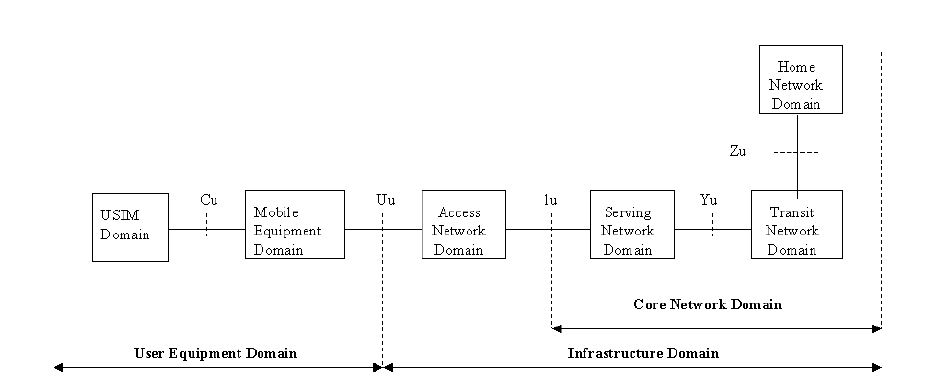
\includegraphics[width=\linewidth]{Kapitel/3G/Grafiken/Domains.jpg}
\captionof{figure}{Übersicht Domains~\cite{3G.1}}
\label{fig:domains}
\end{Figure}

\begin{Figure}
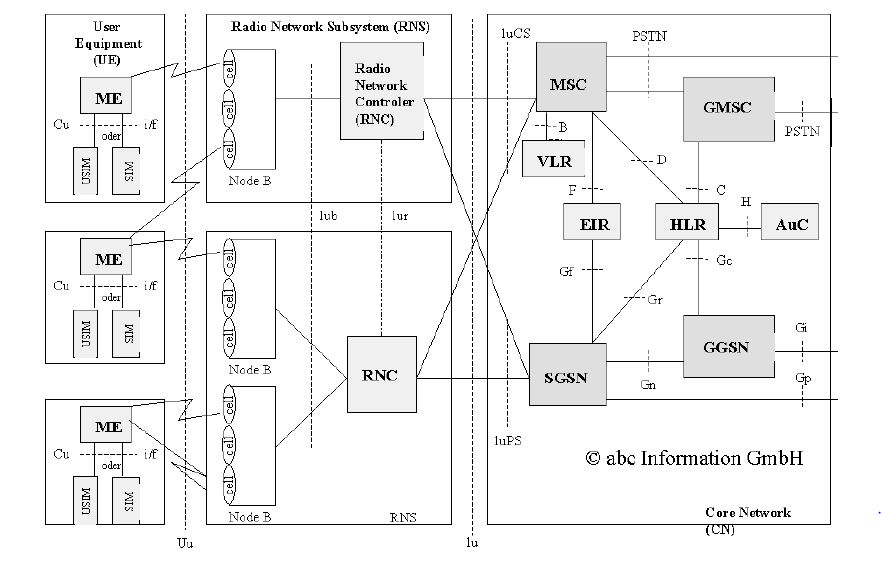
\includegraphics[width=\linewidth]{Kapitel/3G/Grafiken/Architektur.png}
\captionof{figure}{Architektur UMTS ~\cite{3G.1}}
\label{fig:architektur}
\end{Figure}

\end{multicols}

\newpage
\section*{Historische Entwicklung}
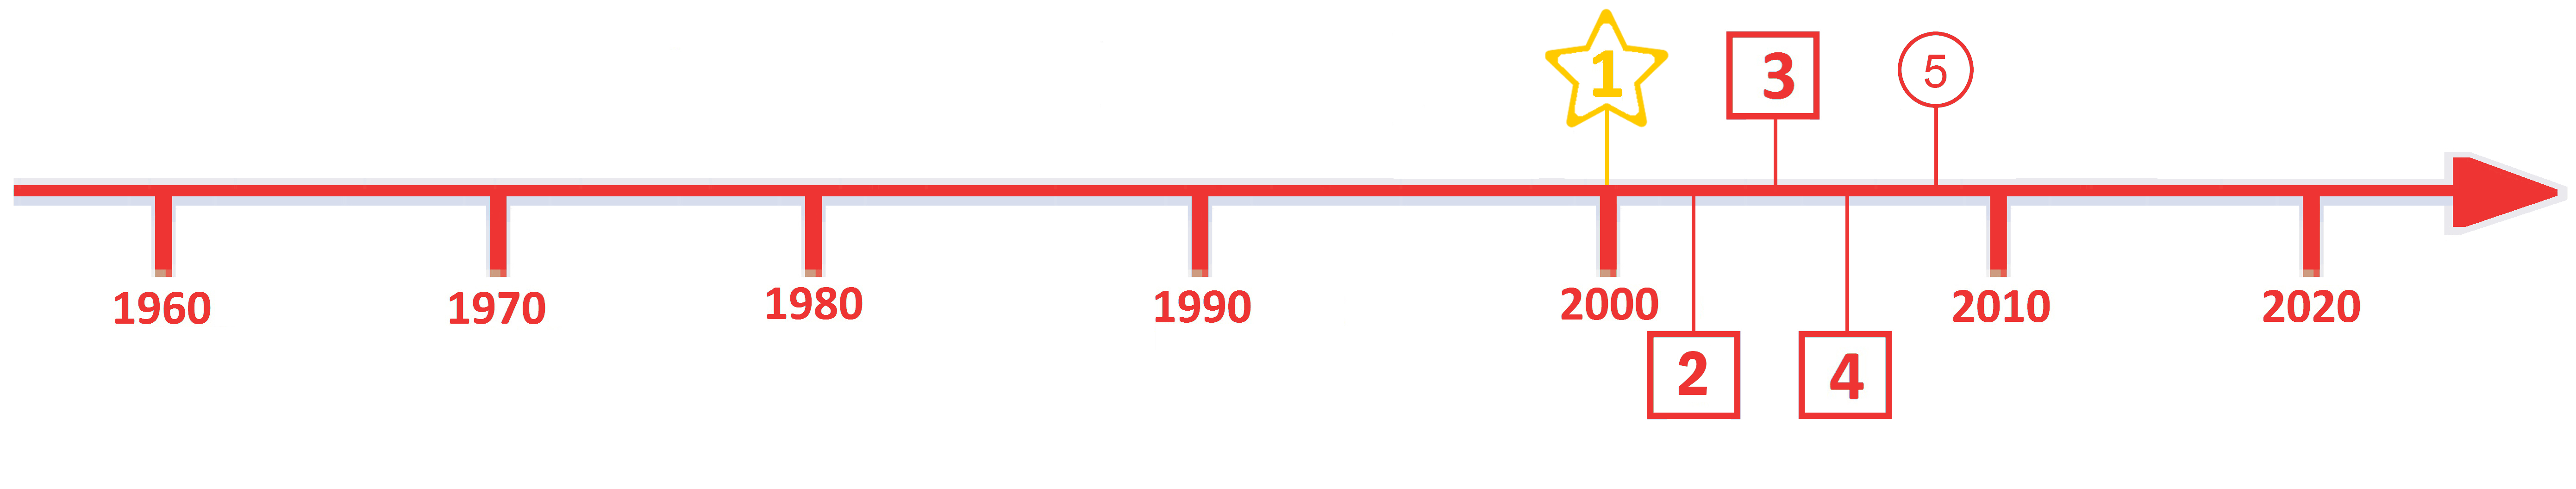
\includegraphics[width=\textwidth]{Kapitel/3G/Grafiken/Zeitstrahl.png}
\par
\noindent
\rowcolors{2}{}{\topicolor!20}
\begin{tabular}{p{0.5 cm}p{1.5 cm}p{15.55 cm}}
	Nr. & Datum & Entwicklungsschritte\\
	1 & 2000 & Einführung von UMTS in den deutschen Markt.\\
	2 & 2004 & Einführung von UMTS fähigen Endgeräten.\\
	3 & 2006 & Einführung von HSDPA in den deutschen Markt.\\
	4 & ab 2007  & Hohe Netzabdeckung von UMTS und HSDPA innerhalb von Deutschland.\\
	5 & 2008 & Eine historische Marke wird erreicht: In Deutschland gibt es nun mehr als 100 Millionen Mobilfunkanschlüsse und damit deutlich mehr Handys als Einwohner.
\end{tabular}
\par
\begin{multicols}{3}

\noindent
Mit dem Protokollzusatz HSDPA kann im Vergleich zu UMTS nun die Leistung einer Funkzelle dauerhaft genutzt werden. Dies wird durch einen neuen Funkkanal erreicht. Eine Erweiterung an den auch sogenannten Basisstationen musst nicht durchgeführt werden, vielmehr musste man bei einigen Basisstationen nur ein Software-Update durchführen.~\cite{3G.8}

\begin{Figure}
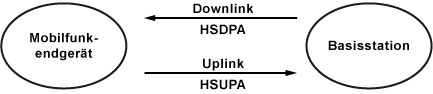
\includegraphics[width=\linewidth]{Kapitel/3G/Grafiken/09102511.png}
\captionof{figure}{Einsatz der Protokolle HSDPA und HSUPA ~\cite{3G.8}}
\label{fig:hsxpa}
\end{Figure}

Die Steuerung des Nutzkanals übernimmt hierbei der \textbf{H}igh \textbf{S}peed \textbf{D}edicated \textbf{P}hysical \textbf{C}ontrol \textbf{C}hannel (\textbf{HS-SCCH}). Durch \textbf{H}igh \textbf{S}peed \textbf{D}ownlink \textbf{S}hared \textbf{C}hannel (\textbf{HS-DSCH}) und \textbf{H}igh \textbf{S}peed \textbf{P}hysical \textbf{S}hared \textbf{C}hannel (\textbf{HS-PSCH}) konnte die verbesserte Übertragungsgeschwindigkeit erreicht werden (siehe Abb. \ref{fig:hsdsch}). 

\begin{Figure}
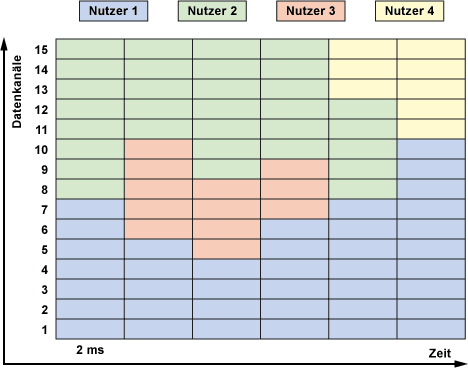
\includegraphics[width=\linewidth]{Kapitel/3G/Grafiken/09102512.png}
\captionof{figure}{Nutzung des HS-DSCH ~\cite{3G.8}}
\label{fig:hsdsch}
\end{Figure}

Auch das \textbf{S}hort \textbf{T}ransmission \textbf{T}ime \textbf{I}nterval (\textbf{STTI}), welches die Zeit für die Übertragung eines Datenpakets beschreibt, konnte um ein Fünftel verringert werden und beträgt somit 2 ms.  Des Weiteren konnte das Multiplexing bei HSDPA durch die Kombination von \textbf{CDMA} (\textbf{C}ode \textbf{D}ivision \textbf{M}ultiple \textbf{A}ccess) und \textbf{TDMA} (\textbf{T}ime \textbf{D}ivision \textbf{M}ultiple \textbf{A}ccess) verbessert werden. Durch die Einteilung der Zeitachse in mehrere Bereiche kann jedem Nutzer ein Zeitbereich bereitgestellt werden. Dieser Bereich hat dann die STTI-Zeitdauer.~\cite{3G.1, 3G.3}

Für den Uplink kann aufgrund der geringen Sendeleistung der Endgeräte nicht die HSDPA-Technik eingesetzt werden. Signale von den Endgeräten kommen mit einer wesentlich schlechteren Qualität an der Basisstation an. Daher kommen robustere Ein-Bit-Modulationsverfahren zum Einsatz, um eine Verbindung zwischen Endgerät und Basisstation herstellen zu können. Diese werden durch den Protokoll-Zusatz HSUPA definiert.~\cite{3G.8}

\subsection*{Einsatz}
Nachdem nun der theoretische Aufbau bekannt ist, folgt eine Erläuterung zum Aufbau einer Sprach- oder Datenverbindung. Zu Beginn muss jedes Mobiletelefon eine SIM-Karte besitzen und sich in einem HLR registrieren. Im nächsten Schritt muss eine Verbindung zu einer Basisstation aufgebaut werden. Dieser Wunsch nach dem Aufbau einer Verbindung leitet die Basisstation weiter zu dem RNC, der diese ebenfalls an den MSC weitergibt. Dort angekommen ordnet der MSC die Telefonnummer dem Nutzer zu und durch Routing kann nun das HLR angesprochen werden. Im Anschluss daran wird die Position, bzw. die Zelle in der sich das Mobilfunkgerät eingewählt hat, dem HLR übermittelt. Der Ort wird im HLR vermerkt und es werden ein Teil der Nutzerdaten an das VLR der aufrufenden MSC gesendet. Nun wird das Mobiltelefon authentifiziert und daraufhin kann ein Telefongespräch mit diesem Gerät geführt werden. Dazu muss nun erneut der Wunsch durch die Basisstation an die RNC und im Anschluss daran an die MSC weitergeleitet werden. Soll nun ein anderes Mobiltelefon angerufen werden, wird dieses durch die HLR aufgerufen, denn dort sind die Positionsdaten gespeichert. Daraufhin kann die Zelle angesprochen werden, indem sich das Mobiltelefon befindet und der Anruf kann getätigt werden. 
Durch den Dezentralen Aufbau dieses Netzes kann ein Gesamtausfall vermieden werden, da höchstens Teilgebiete des Mobilfunkproviders ausfallen können. ~\cite{3G.1}

\subsection*{Anbieter und Gremien}
Wie in den vorherigen Abschnitten bereits beschrieben, waren die Firmen für den Netzausbau verantwortlich, die die Lizenzen für UMTS erworben haben. Dies waren die Firmen \textit{T-Mobile Deutschland GmbH}, \textit{Vodafone D2 GmbH}, \textit{MobilCom Multimedia GmbH, Auditorium Investments Germany S.à.r.l.} (später umformiert in \textit{E-plus 3G Luxemburg S.à.r.l.}), \textit{O2} und \textit{Group 3G} (ein Konsortium aus der spanischen \textit{Telefónica} und der finnischen \textit{Sonera}). In den Folgejahren gaben die Firmen \textit{MobilCom Multimedia GmbH} und \textit{Group 3G} ihre Lizenzen wieder ab.
Die HSPA Netzanbieter von Deutschland sind \textit{T-Mobile}, \textit{Vodafone}, \textit{o2} und \textit{E-Plus}. Alle bekannten Anbieter von 3G Tarifen nutzen das Netz einer dieser Provider. 
~\cite{3G.1, 3G.2}

\subsection*{Ausblick}
Der nächste Schritt in der evolutionären Entwicklung des mobilen Internets ist 4G oder auch LTE (Long Term Evolution) genannt. Mitte August des Jahres 2010 wurde in Deutschland der erste LTE-Sendemast errichtet. Aber nähere Erläuterungen zu LTE finden Sie im folgenden Artikel ~\cite{3G.2}.

\printbibliography[segment=8,heading=subbibliography]
\end{multicols}

\newpage
